\documentclass[a4paper,12pt]{article}
\usepackage[brazil]{babel} 
\usepackage[utf8]{inputenc} 

\usepackage{amssymb}
\usepackage{algorithm}
\usepackage{algpseudocode}
\usepackage{geometry}
\usepackage{longtable}
\usepackage{indentfirst} 
\usepackage{listings}
\usepackage{color}
\usepackage{graphicx}
\usepackage{url}

% ---
% Configurações de Listings
% ---
\definecolor{mygreen}{rgb}{0,0.6,0}
\definecolor{mygray}{rgb}{0.5,0.5,0.5}
\definecolor{mymauve}{rgb}{0.58,0,0.82}
\definecolor{codegreen}{rgb}{0,0.6,0}
\definecolor{codegray}{rgb}{0.5,0.5,0.5}
\definecolor{codepurple}{rgb}{0.58,0,0.82}
\definecolor{backcolour}{rgb}{0.95,0.95,0.92}
\lstset{
	backgroundcolor=\color{white},   % choose the background color; you must add \usepackage{color} or \usepackage{xcolor}
	basicstyle=\footnotesize,        % the size of the fonts that are used for the code
	breakatwhitespace=false,         % sets if automatic breaks should only happen at whitespace
	breaklines=true,                 % sets automatic line breaking
	captionpos=b,                    % sets the caption-position to bottom
	commentstyle=\color{mygreen},    % comment style
	deletekeywords={...},            % if you want to delete keywords from the given language
	escapeinside={\%*}{*)},          % if you want to add LaTeX within your code
	extendedchars=true,              % lets you use non-ASCII characters; for 8-bits encodings only, does not work with UTF-8
	keepspaces=true,                 % keeps spaces in text, useful for keeping indentation of code (possibly needs columns=flexible)
	keywordstyle=\color{blue},       % keyword style
	language=C,                      % the language of the code
	otherkeywords={*,...},           % if you want to add more keywords to the set
	numbers=left,                    % where to put the line-numbers; possible values are (none, left, right)
	numbersep=5pt,                   % how far the line-numbers are from the code
	numberstyle=\tiny\color{mygray}, % the style that is used for the line-numbers
	rulecolor=\color{black},         % if not set, the frame-color may be changed on line-breaks within not-black text (e.g. comments (green here))
	showspaces=false,                % show spaces everywhere adding particular underscores; it overrides 'showstringspaces'
	showstringspaces=false,          % underline spaces within strings only
	showtabs=false,                  % show tabs within strings adding particular underscores
	stepnumber=1,                    % the step between two line-numbers. If it's 1, each line will be numbered
	stringstyle=\color{mymauve},     % string literal style
	tabsize=2,	                   % sets default tabsize to 2 spaces
	title=\lstname                   % show the filename of files included with \lstinputlisting; also try caption instead of title
}
% ---

\algnewcommand\algorithmicforeach{\textbf{for each}}
\algdef{S}[FOR]{ForEach}[1]{\algorithmicforeach\ #1\ \algorithmicdo}


\begin{document} 



\begin{titlepage}

\newcommand{\HRule}{\rule{\linewidth}{0.5mm}} % Defines a new command for the horizontal lines, change thickness here

\center % Center everything on the page


%----------------------------------------------------------------------------------------
%	HEADING SECTIONS
%----------------------------------------------------------------------------------------

\textsc{\LARGE Universidade Federal\\do Espírito Santo}\\[1.5cm] % Name of your university/college
\textsc{\Large Centro Tecnológico}\\[0.5cm] % Major heading such as course name
\textsc{\large Departamento de Informática}\\[0.5cm] % Minor heading such as course title

%----------------------------------------------------------------------------------------
%	TITLE SECTION
%----------------------------------------------------------------------------------------

\HRule \\[0.4cm]
{ \huge \bfseries Job Scheduler}\\[0.4cm] % Title of your document
\HRule \\[1.5cm]

%----------------------------------------------------------------------------------------
%	AUTHOR SECTION
%----------------------------------------------------------------------------------------

\begin{minipage}{0.4\textwidth}
\begin{flushleft} \large
\emph{Autor:}\\
Vinicius \textsc{Arruda}
\end{flushleft}
\end{minipage}
~
\begin{minipage}{0.4\textwidth}
\begin{flushright} \large
\emph{Professora:} \\
Mariella \textsc{Berger} % Supervisor's Name
\end{flushright}
\end{minipage}\\[2cm]

% If you don't want a supervisor, uncomment the two lines below and remove the section above
%\Large \emph{Author:}\\
%John \textsc{Smith}\\[3cm] % Your name

%----------------------------------------------------------------------------------------
%	LOGO SECTION
%----------------------------------------------------------------------------------------


\includegraphics[width=58mm]{LogoUfes.png}\\[1cm] % Include a department/university logo - this will require the graphicx package

%----------------------------------------------------------------------------------------
%----------------------------------------------------------------------------------------
%	DATE SECTION
%----------------------------------------------------------------------------------------

{\large 10 de outubro de 2015}\\[2cm] % Date, change the \today to a set date if you want to be precise

\vfill % Fill the rest of the page with whitespace

\end{titlepage}





\begin{abstract}
Trabalho da disciplina de Estrutura de Dados II, que consiste na implementação 
de dois algoritmos para solucionar o problema de escalonamento de tarefas (do inglês: \textit{Job Scheduler}). Os 
algoritmos são o Beam Search e o Branch and Bound.
\end{abstract}

\newpage






\section{Introdução} % Este comando faz o tíıtulo da seção.
%INTRODUÇÃO

Um escalonador de tarefas é um programa que consiste em determinar uma atribuição de tarefas para um processador
de forma a otimizar o tempo de execução total destas tarefas. O problema de um escalonador de tarefas é da classe dos 
problemas NP-completo (do inglês: \textit{NP-complete}) e pode ser convertido para o problema da 
mochila (do inglês: \textit{knapsack problem}) e do caixeiro viajante (do inglês: \textit{travelling salesman problem}).

A proposta deste trabalho é mostrar duas implementações para encontrar o melhor escalonamento de tarefas. O Beam Search 
é uma das implementações, e por se tratar de uma heurística, o resultado não é necessariamente o melhor. A outra 
implementação é o Branch and Bound, que é um algoritmo exato e encontra o melhor escalonamento.

%OBJETIVO:
\section{Objetivo}
Aplicar o conhecimento adquirido na disciplina de Estruturas de Dados II e reconhecer a complexidade dos 
problemas NP-completo aplicando algoritmos de aproximação e outras técnicas para contornar a dificuldade do 
problema em encontrar a solução ótima.

%FERRAMENTAS:
\section{Ferramentas}
Os algoritmos foram implementados na linguagem de programação C. Para a compilação foi 
utilizado o compilador GCC versão 4.8.4 em uma máquina com o sistema operacional Ubuntu 14.04.3.
O código foi escrito utilizando o editor de texto Sublime Text.
Para a depuração do programa, foi utilizado a ferramenta Valgrind versão 3.10.


\section{Beam Search}
Beam Search é uma heurística de busca que explora um grafo expandindo o caminho mais promissor. No caso deste 
trabalho, o caminho mais promissor é aquele de menor \emph{Upper Bound}\footnote{\emph{Upper Bound}: Cálculo 
feito a priori do custo máximo que um caminho pode obter. A medida que o caminho vai sendo percorrido, este 
valor pode decrescer.}. O Beam Search explora o grafo em largura (do inglês: \textit{Breadth-first Search}) 
montando uma árvore. A cada nível da árvore montada, o algoritmo gera os filhos dos \emph{n} nós mais promissores, 
onde \emph{n} é o \emph{Beam-width}\footnote{\emph{Beam-width}: Número de nós promissores a serem desenvolvidos.} e 
todos os outros nós são descartados. Escolher o nó de menor \emph{Upper Bound} não garante que este produzirá a 
melhor solução, por isso, se trata de uma heurística.

\subsection{Metodologia}

Inicialmente, uma implementação do Beam Search baseada em busca primeiro em profundidade (do inglês: 
\textit{Depth-first Search}) foi desenvolvida. Após algumas pesquisas sobre o Beam Search para a elaboração deste 
relatório, foi constatado que este deveria ser implementado baseado em busca primeiro em largura. Sendo assim, 
uma outra versão foi implementada baseado na busca primeiro em largura.

No arquivo \emph{beamSearch.c} na pasta \emph{BeamSearch}, encontra-se a implementação das duas versões com as assinaturas 
\emph{beamSearchBreadth(...)} e \emph{beamSearchDepth(...)} para a versão em busca primeiro em largura e busca 
primeiro em profundidade, respectivamente. A versão utilizada ao executar \emph{./trab3 \# bs} é a baseada em busca 
primeiro em largura, pois de acordo com a pesquisa feita\footnote{Ver referências no final do relátório.} e com os testes realizados, o resultado é 
obtido mais rápido e com melhor precisão.


\begin{algorithm}[H]
\caption{Função de auxiliar ao Beam Search} \label{HandlerBS}
\begin{algorithmic}[1]
\Function{Handler}{PriorityQueue, E, s, BeamWidth} 
\ForEach {$b \in E $}
\State $\textit{CalculatesBoundaries}(b)$  \Comment{Calculates the lower and upper bound of b.}
\If {$ b.LowerBound < s.Cost $}
	\If {$ b.UpperBound < s.Cost $} 
		\State $s.Cost \gets b.UpperBound$
	\EndIf
	\\
	\If {$ b.LowerBound = b.UpperBound $} 
		\If {$ b.UpperBound = s.Cost $} 
			\State $s \gets b$
		\EndIf
	\Else
		\State $PriorityQueue.\textit{Enqueue}(b)$
	\EndIf
\EndIf
\EndFor 
\State $PriorityQueue.\textit{Reduce}(BeamWidth)$    \Comment{Reduces the Queue to BeamWidth elements.}
\EndFunction
\end{algorithmic}
\end{algorithm}


O algoritmo \ref{HandlerBS} mostra uma função que é utilizada no código do Beam Search para manipular o 
\emph{Lower Bound} e o \emph{Upper Bound} de cada nó e a partir de seus valores, decidir se será incluso 
na fila de prioridade ou se sera excluído. A exclusão de um nó se ocorre quando o custo do caminho chegando 
até este for maior que o custo do melhor caminho encontrado ou quando a fila já possuir \emph{Beam-width} 
elementos de maior prioridade.

A seguir, o algoritmo \ref{AlgoritmoBSDFS} representa a primeira implementação do Beam Search, baseado 
em busca primeiro em profundidade e logo após, o algoritmo \ref{AlgoritmoBSBFS} que é a implementação atual, 
baseada em busca primeiro em largura.


\begin{algorithm}[H]
\caption{Algoritmo Beam Search baseado em Depth-first Search} \label{AlgoritmoBSDFS}
\begin{algorithmic}[1]
\Procedure{BeamSearchDepth}{Jobs, BeamWidth}
\State $s \gets \infty$                       \Comment{Best solution.}
\State $C \gets \varnothing$                       \Comment{Set of nodes generated by a promising node.} 
\State $PriorityQueue \gets \varnothing$  
\State $J \gets Jobs$
\State $\textit{Handler}(PriorityQueue, J, s, BeamWidth)$
\While{$PriorityQueue \neq \varnothing$}
\State $j \gets PriorityQueue.\textit{Dequeue}()$
\State $C \gets \textit{Explore}(j)$                \Comment{Return the children nodes of j.}
\State $\textit{Handler}(PriorityQueue, C, s, BeamWidth)$
\EndWhile
\EndProcedure
\end{algorithmic}
\end{algorithm}


\begin{algorithm}[H]
\caption{Algoritmo Beam Search baseado em Breadth-first Search} \label{AlgoritmoBSBFS}
\begin{algorithmic}[1]
\Procedure{BeamSearchBreadth}{Jobs, BeamWidth}
\State $s \gets \infty$                       \Comment{Best solution.}
\State $C \gets \varnothing$                       \Comment{Set of nodes generated by a promising node.} 
\State $PrevPQ \gets \varnothing$                  \Comment{Previous level Priority Queue.} 
\State $NextPQ \gets \varnothing$                  \Comment{Next level Priority Queue.} 
\State $J \gets Jobs$
\State $\textit{Handler}(PrevPQ, J, s, BeamWidth)$

\While {$PrevPQ \neq \varnothing$}
	\While {$PrevPQ \neq \varnothing$}
		\State $j \gets PriorityQueue.\textit{Dequeue}()$
		\State $C \gets \textit{Explore}(j)$                \Comment{Return the children nodes of j.}
		\State $\textit{Handler}(NextPQ, C, s, BeamWidth)$
	\EndWhile
	\State $PrevPQ \gets NextPQ$
	\State $NextPQ \gets \varnothing$
\EndWhile
\EndProcedure
\end{algorithmic}
\end{algorithm}




\subsection{Resultados}

Para analisar os resultados, foi elaborado um script para criar Jobs aleatórios. Os Jobs foram gerados com 
números aleatórios de 1 a 1000, sendo que o valor da \emph{deadline} é sempre maior ou igual ao valor do tempo 
de processamento.

Foram gerados um total de 100 arquivos de Jobs, cada um com um número de Jobs distinto, indo de 10 à 1000, de 10 em 10.
Para a análise do \emph{Beam Width}, foi executado para cada arquivo de Jobs o algoritmo Beam Search nas duas versões, 
com o \emph{Beam Width} indo de 1 à 15 de 2 em 2, e de 20 à 50 de 5 em 5, somando um total de 15 valores de 
\emph{Beam Width} distintos para cada arquivo de Jobs.

O resultado final da base de testes para as configurações dispostas acima gerou uma tabela de 1500 linhas por 7 colunas, 
e a partir dela foi gerada uma outra tabela filtrando apenas os resultados dos melhores custos para cada arquivo de Jobs.
O resultado filtrado se encontra na tabela \ref{tabelaBS} a seguir.


\begin{center} 
\newgeometry{left=1cm,right=1cm,top=0.5cm,bottom=0.5cm} 
\begin{longtable}{|c|c|c|c|c|c|c|} 
\caption{Resultados do algoritmo Beam Search.} \label{tabelaBS}\\  
\hline
\multicolumn{1}{c}{} & \multicolumn{3}{c}{Breadth-first Search} & \multicolumn{3}{c}{Depth-first Search}\\
\hline
\textbf{\# Jobs} & \textbf{Beam Width} & \textbf{Custo} & \textbf{Tempo (s)} & \textbf{Beam Width} & \textbf{Custo} 
& \textbf{Tempo (s)} \\
\hline
\endfirsthead
\multicolumn{7}{c}%
{\tablename\ \thetable\ -- \textit{Continuação - Resultados do algoritmo Beam Search.}} \\
\hline
\multicolumn{1}{c}{} & \multicolumn{3}{c}{Breadth-first Search} & \multicolumn{3}{c}{Depth-first Search}\\
\hline
\textbf{\# Jobs} & \textbf{Beam Width} & \textbf{Custo} & \textbf{Tempo (s)} & \textbf{Beam Width} & \textbf{Custo} 
& \textbf{Tempo (s)} \\
\hline
\endhead
\hline \multicolumn{7}{c}{\textit{Continua na próxima página.}} \\
\endfoot
\hline
\endlastfoot
10   &   1   &   2116   &   0   &   1   &   2116   &   0  \\
20   &   30   &   5407   &   0   &   35   &   5159   &   0.006  \\
30   &   5   &   14688   &   0   &   35   &   14688   &   0  \\
40   &   25   &   18222   &   0   &   45   &   18222   &   0.029  \\
50   &   25   &   23541   &   0.003   &   30   &   23998   &   0.015  \\
60   &   20   &   24547   &   0.004   &   50   &   25421   &   0.599  \\ 
70   &   9   &   29805   &   0.003   &   40   &   32563   &   0.028  \\
80   &   25   &   39013   &   0.008   &   30   &   39537   &   0.023  \\
90   &   30   &   37638   &   0.015   &   1   &   40072   &   0  \\
100   &   25   &   43635   &   0.018   &   35   &   45216   &   2.231  \\
110   &   30   &   50427   &   0.028   &   1   &   53666   &   0  \\
120   &   20   &   59167   &   0.019   &   20   &   59167   &   0.063  \\
130   &   35   &   55347   &   0.033   &   30   &   56458   &   0.026  \\
140   &   5   &   64308   &   0.007   &   1   &   68389   &   0  \\
150   &   45   &   65546   &   0.091   &   1   &   72327   &   0  \\
160   &   35   &   71099   &   0.093   &   5   &   76897   &   0  \\
170   &   20   &   73427   &   0.036   &   1   &   76482   &   0  \\
180   &   50   &   81370   &   0.103   &   35   &   85193   &   0.149  \\
190   &   45   &   88590   &   0.105   &   45   &   90713   &   0.43  \\
200   &   25   &   98563   &   0.06   &   45   &   103045   &   1.798  \\
210   &   20   &   94139   &   0.06   &   1   &   97490   &   0.004  \\
220   &   20   &   105507   &   0.062   &   45   &   107596   &   2.842  \\
230   &   1   &   107203   &   0.004   &   1   &   107203   &   0.004  \\
240   &   50   &   113709   &   0.172   &   50   &   116441   &   2.825  \\
250   &   30   &   116825   &   0.136   &   1   &   123111   &   0.003  \\
260   &   50   &   121388   &   0.25   &   1   &   122990   &   0.005  \\
270   &   35   &   119963   &   0.195   &   35   &   124032   &   0.26  \\
280   &   15   &   125289   &   0.126   &   1   &   131814   &   0.006 \\  
290   &   15   &   137340   &   0.088   &   1   &   143029   &   0.004  \\
300   &   3   &   144936   &   0.019   &   1   &   146246   &   0.006 \\
310   &   13   &   144254   &   0.133   &   25   &   148236   &   0.286 \\
320   &   50   &   156292   &   0.339   &   1   &   159100   &   0.008  \\ 
330   &   15   &   154338   &   0.121   &   1   &   161481   &   0.005  \\
340   &   50   &   163944   &   0.397   &   1   &   168758   &   0.008  \\
350   &   7   &   162199   &   0.067   &   1   &   165264   &   0.009  \\
360   &   30   &   184675   &   0.246   &   20   &   187477   &   0.333  \\
370   &   7   &   174647   &   0.070   &   20   &   175874   &   0.705  \\
380   &   25   &   176947   &   0.236   &   1   &   180560   &   0.008  \\
390   &   20   &   185904   &   0.292   &   1   &   194711   &   0.005  \\
400   &   3   &   193068   &   0.026   &   1   &   195792   &   0.011  \\
410   &   15   &   183211   &   0.278   &   30   &   191137   &   2.355  \\
420   &   20   &   217921   &   0.252   &   1   &   221013   &   0.012  \\
430   &   50   &   199521   &   1.232   &   1   &   206763   &   0.01  \\
440   &   5   &   219350   &   0.075   &   1   &   222770   &   0.011  \\
450   &   7   &   205101   &   0.135   &   1   &   211827   &   0.013  \\
460   &   1   &   231464   &   0.017   &   1   &   231464   &   0.017  \\
470   &   11   &   224489   &   0.22   &   1   &   229975   &   0.012  \\
480   &   35   &   224341   &   0.942   &   1   &   231341   &   0.011  \\
490   &   25   &   235094   &   0.593   &   1   &   240679   &   0.013  \\
500   &   25   &   239052   &   0.581   &   1   &   243407   &   0.015  \\
510   &   25   &   239110   &   0.484   &   1   &   248254   &   0.014  \\ 
520   &   11   &   254474   &   0.236   &   1   &   259434   &   0.017  \\
530   &   25   &   249127   &   0.59   &   1   &   255166   &   0.012  \\
540   &   40   &   251451   &   0.863   &   1   &   254037   &   0.024  \\
550   &   25   &   268296   &   0.508   &   1   &   274419   &   0.01  \\
560   &   5   &   273821   &   0.125   &   1   &   275817   &   0.028  \\
570   &   25   &   273539   &   0.819   &   1   &   277508   &   0.024  \\
580   &   7   &   284812   &   0.196   &   1   &   288250   &   0.021  \\
590   &   20   &   281137   &   0.57   &   1   &   289789   &   0.012  \\
600   &   11   &   289618   &   0.39   &   1   &   298223   &   0.017  \\
610   &   25   &   294442   &   0.88   &   1   &   304456   &   0.014  \\
620   &   15   &   291908   &   0.71   &   1   &   297302   &   0.031  \\
630   &   7   &   306224   &   0.292   &   1   &   312330   &   0.014  \\
640   &   50   &   314449   &   2.041   &   30   &   320320   &   2.323  \\
650   &   9   &   320060   &   0.34   &   1   &   322588   &   0.033  \\
660   &   40   &   337446   &   1.727   &   1   &   342969   &   0.027  \\
670   &   40   &   331950   &   1.648   &   1   &   333809   &   0.032  \\
680   &   35   &   332758   &   2.477   &   1   &   338038   &   0.043  \\
690   &   7   &   333156   &   0.254   &   1   &   335149   &   0.032  \\
700   &   30   &   331872   &   1.611   &   1   &   337818   &   0.028  \\
710   &   9   &   346765   &   0.49   &   1   &   349552   &   0.036  \\
720   &   40   &   356180   &   2.006   &   1   &   365181   &   0.023  \\
730   &   20   &   361947   &   0.993   &   1   &   365545   &   0.048  \\
740   &   7   &   377962   &   0.326   &   1   &   379822   &   0.035  \\
750   &   40   &   381025   &   2.646   &   1   &   386714   &   0.039  \\
760   &   45   &   364211   &   3.501   &   1   &   366620   &   0.054  \\
770   &   50   &   377252   &   2.24   &   1   &   385433   &   0.017  \\
780   &   40   &   374846   &   2.247   &   3   &   380221   &   0.056  \\
790   &   40   &   388331   &   3.363   &   1   &   395538   &   0.035  \\
800   &   20   &   392043   &   1.091   &   1   &   396963   &   0.043  \\
810   &   20   &   389193   &   1.539   &   1   &   399469   &   0.027  \\
820   &   45   &   406499   &   2.754   &   1   &   414759   &   0.048  \\
830   &   40   &   409492   &   2.084   &   1   &   412812   &   0.034  \\
840   &   40   &   405288   &   2.823   &   1   &   413555   &   0.025  \\
850   &   40   &   410465   &   3.308   &   1   &   416220   &   0.069  \\
860   &   25   &   420828   &   1.794   &   1   &   427606   &   0.079  \\
870   &   20   &   438434   &   1.799   &   1   &   441639   &   0.143  \\
880   &   9   &   435297   &   0.831   &   1   &   441932   &   0.092  \\
890   &   20   &   432000   &   2.164   &   1   &   439794   &   0.071  \\
900   &   50   &   442968   &   3.669   &   35   &   447016   &   14.005  \\
910   &   25   &   453157   &   2.235   &   1   &   457580   &   0.111  \\
920   &   30   &   446557   &   2.944   &   1   &   452133   &   0.088  \\
930   &   45   &   452940   &   5.184   &   1   &   459833   &   0.144  \\
940   &   3   &   467678   &   0.273   &   1   &   470033   &   0.081  \\
950   &   20   &   473669   &   2.251   &   1   &   482473   &   0.067  \\
960   &   40   &   458785   &   5.531   &   1   &   465562   &   0.115  \\
970   &   25   &   456365   &   2.627   &   1   &   465185   &   0.071  \\
980   &   7   &   487925   &   0.625   &   1   &   494015   &   0.121  \\
990   &   40   &   474197   &   5.629   &   1   &   485967   &   0.115  \\
1000   &   11   &   477882   &   1.097   &   1   &   484289   &   0.051  \\

\end{longtable}

\restoregeometry%get the old one pack

\end{center}


Podemos observar pela tabela \ref{tabelaBS} a quantidade de melhores soluções que cada versão obteve, 
e segue na tabela \ref{QbestSolution}.

\begin{table}[H]
\centering
\caption{Quantidade de melhor solução para as duas versões.} \label{QbestSolution}
\begin{tabular}{ccc}
\hline
Breadth-first Search & Depth-first Search & Ambas as versões \\
\hline
  93 & 1  &  6  \\
\hline
\end{tabular}
\end{table}


Ainda pela tabela \ref{tabelaBS}, obtemos o número de soluções encontradas para cada \emph{Beam Width} 
da tabela e segue o resultado na tabela \ref{NumBestSol}.


\begin{table}[H]
\centering
\caption{Número de melhores soluções para cada Beam Width.} \label{NumBestSol}
\begin{tabular}{ccc}
\hline
Beam Width & Número de soluções \\
\hline
1  &  3  \\
3  &  3  \\
5  &  4  \\
7  &  8  \\
9  &  4  \\
11  &  4  \\
13  &  1  \\
15  &  5  \\
20  &  14  \\
25  &  16  \\
30  &  6  \\
35  &  6  \\
40  &  12  \\
45  &  5  \\
50  &  9  \\
\hline
\end{tabular}
\end{table}


\subsection{Conclusão}

A partir dos resultados obtidos, configuramos como \emph{Beam Width} do algoritmo Beam Search o valor 25, pois 
pela tabela \ref{NumBestSol}, com este valor o algoritmo Beam Search obteve melhores soluções.

Não podemos, de forma alguma generalizar o \emph{Beam Width} 25 como melhor \emph{Beam Width} possível, pois pela 
natureza do algoritmo, ele é sensível a entrada. Mas podemos admitir que 25 é um bom valor de \emph{Beam Width}.

Sem dúvidas o Beam search baseado em busca primeiro em largura se mostrou muito mais eficiente do que o baseado 
em busca primeiro em profundidade. O lado negativo do baseado em busca primeiro em largura é um maior consumo de 
memória para um \emph{Beam Width} muito grande, mas para valores como 100, a memória gasta é irrelevante.


\newpage

\section{Branch and Bound}

Branch and bound é um algoritmo que busca o valor exato, ou seja, o melhor valor possível para o problema. 
É mais lento que o Beam Search por precisar percorrer varias possibilidades. O Branch and Bound 
consiste em uma enumeração sistemática de todos os candidatos à solução, com a eliminação de um candidato parcial à 
solução quando puder ser afirmado que esta não será a melhor escolha. 
Dependendo do tamanho da entrada, torna-se inviável nos piores casos utilizar o Branch and Bound.
O desempenho do algoritmo Branch and Bound está fortemente relacionado a qualidade dos seus limitantes inferiores 
e superiores (Lower Bound e Upper Bound), quanto mais precisos forem estes limitantes, menos soluções parciais 
serão consideradas e mais rápido o algoritmo encontrará a solução ótima.

A forma encontrada para não cair no pior caso é utilizar uma heurística antes e a partir do resultado dela realizar 
o algoritmo, assim melhorando significantemente o tempo de execução do programa gerando soluções razoavelmente rápidas 
nos casos médios. Para este trabalho, o algoritmo Beam Search será a heurística que fornecerá uma possível solução para 
o problema do escalonamento de tarefas, e a partir desta solução, o algoritmo Branch and Bound irá procurar e encontrar 
a melhor solução possível.


A figura abaixo mostra um pequeno exemplo de 3 Jobs. Caso o Branch and Bound tenha como solução inicial 
fornecido por uma heurística o valor 9, as ramificações serão como o da figura. Podemos garantir que o custo 
de qualquer escalonamento que comece com os Jobs 0 depois 2 tenha o custo 6, então é só preencher o escalonamento 
com os Jobs que restam, que no caso é o Job 1. Então o escalonamento de menor custo encontrado é: 0 2 1, com custo 
6.

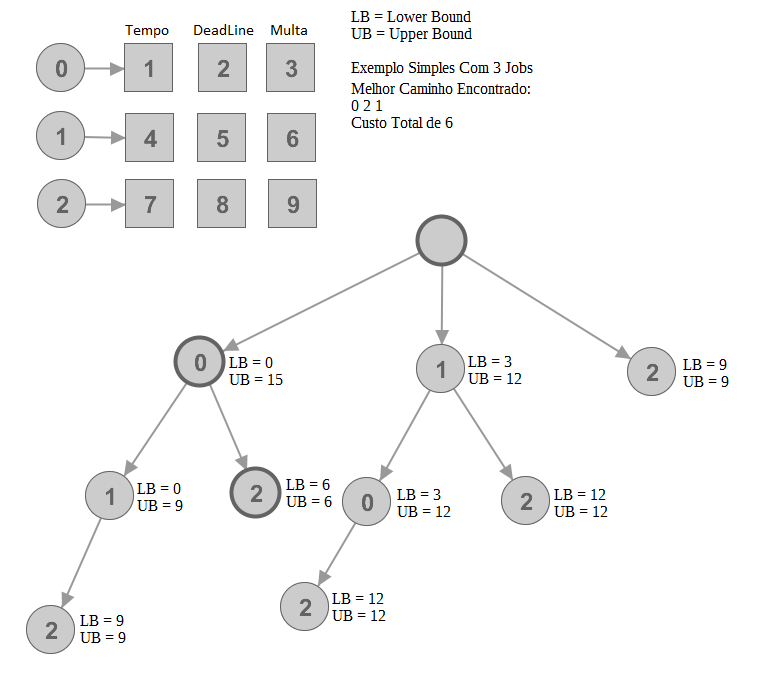
\includegraphics[width=145mm]{bb.png}\\[1cm] \label{bbimg}

\subsection{Metodologia}

A meodologia para o Branch and Bound é semelhante ao Beam Search, porém se fosse possível, seria equivalente 
a utilizar o Beam Search com o valor infinito para o \emph{Beam Width}.
Para o Branch and Bound, apesar de ter sido implementado, se manteve apenas a implementação baseada em 
busca primeiro em profundidade, pois para o baseado em busca primeiro em largura, o consumo de memória cresce 
a medida que as ramificações crescem, e para os casos médios a ruins, isso pode ser até fatorial. Utilizando 
uma base de testes de 40 Jobs e uma implementação do Branch and Bound baseado em busca primeiro em largura 
a execução consumiu em menos de um minuto 5 GigaBytes de memória.

Uma observação importante a se fazer é ter uma boa implementação de uma fila de prioridade. Esta fila seria útil 
para o Beam Search e principalmente para o Branch and Bound. Neste trabalho, foi utilizado uma implementação 
ineficiente para a fila de prioridade, uma lista encadeada ordenada.

Durante a execução da base de testes, se mostrou bastante necessário uma boa fila de prioridade, mas, mesmo se 
o problema cair em um caso médio à ruim, uma boa fila de prioridade não terá grande diferença, pois sua 
complexidade pode ser fatorial para o pior caso.


\subsection{Resultados}

Infelizmente, várias base de testes caíram em casos ruíns, onde a solução do Beam Search não foi muito boa ou 
a entrada de dados era muito ruim, pois pode haver casos em que uma grande quantidade de ramificações pode ser 
gerada.
As bases de testes foram executadas de 3 em 3, pois a máquina em que foi executado o algoritmo possue 4 núcleos, 
e essas 3 bases ocupariam 3 núcleos. 
As bases de 60 Jobs e de 100 Jobs por exemplo, executaram por mais de 12 horas, e não concluíram o processamento 
até a entrega deste relatório.
A base de 80 Job executou por mais de 5 horas e também não concluiu o processamento.

O resultado obtido pode ser visto na tabela \ref{BB}, onde faz um comparativo do valor encontrado pela heurística 
e o valor encontrado pelo Branch and Bound.
Podemos observar também, que em alguns casos a heurística Beam Search pode encontrar a solução exata do problema.


\begin{table}[H]
\centering
\caption{Resultado Branch and Bound} \label{BB}
\begin{tabular}{cccc}
\hline
\# Jobs & Solução Beam Search & Solução Branch and Bound & tempo (s) \\
\hline
	10 & 2116 & 2116 & 0.000 \\
	20 & 5407 & 5159 & 0.069 \\
	30 & 14688 & 14688 & 0.006 \\
	40 & 18222 & 17786 & 0.459 \\
	50 & 23541 & 22926 & 3.434 \\
\hline
\end{tabular}
\end{table}




\newpage

%REFERÊNCIAS BIBLIOGRÁFICAS:
\section{Referências Bibliográficas}
\begin{enumerate}
\item \url{http://www.ic.unicamp.br/~zanoni/mc102/2013-1s/aulas/aula22.pdf} 
\item \url{https://pt.wikipedia.org/wiki/Branch_and_bound} 
\item \url{https://en.wikipedia.org/wiki/Beam_search} 
\item \url{https://en.wikibooks.org/wiki/Artificial_Intelligence/Search/Heuristic_search/Beam_search} 
\item \url{http://www.win.tue.nl/~awijs/articles/beam.pdf}
\item \url{https://www.aaai.org/Papers/AAAI/1998/AAAI98-060.pdf} 
\end{enumerate}


\end{document}



